\chapter{Исследовательская часть}

В данном разделе будут приведены результаты работы разработанного программного обеспечения и поставлен эксперимент по сравнению уровня и характера шума синтезируемого изображения с использование классическом алгоритма (метода Монте - Карло) и квантового алгоритма избыточной выборки на различных размерах изображения.

\section{Результаты работы программного обеспечения}

На рисунке \ref{img:reference} приведенно эталонное изображение, с которого будет проводиться избыточная выборка.

\begin{figure}[H]
	\begin{center}
		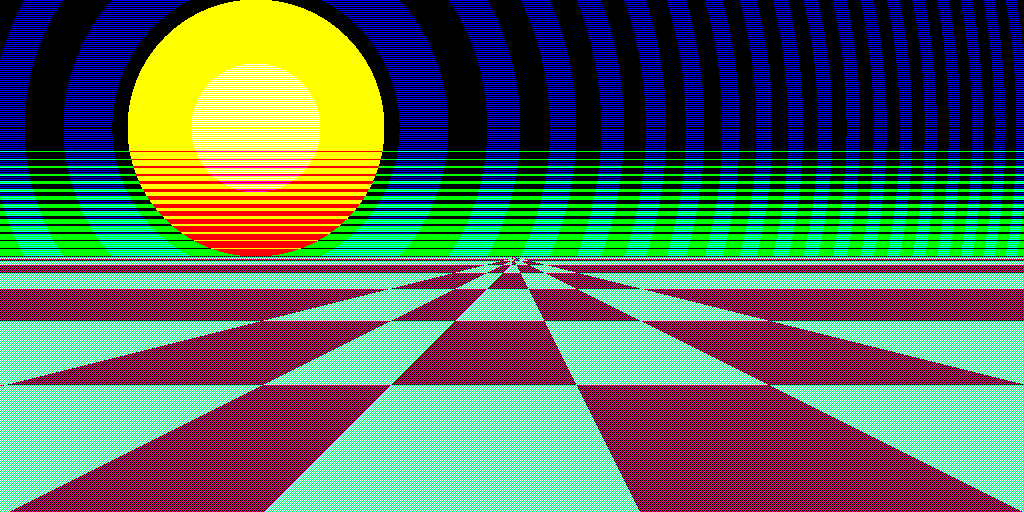
\includegraphics[scale=0.48]{img/prog_res/reference-1024.png}
	\end{center}
	\captionsetup{justification=centering}
	\caption{Эталонное изображение размером 1024х512}
	\label{img:reference}
\end{figure}

На изображении \ref{img:example_01} - \ref{img:example_03-mc} приведен результат работы ПО для разных размеров изображений. 

\begin{figure}[H]
	\begin{center}
		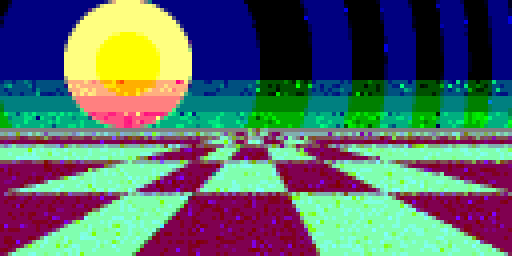
\includegraphics[scale=0.96]{img/prog_res/qss-512-4.png}
	\end{center}
	\captionsetup{justification=centering}
	\caption{Результат работы квантового алгоритма, 512х256, 4 итераций увеличения комплексной амплитуды, размер сабпикселя 4х4}
	\label{img:example_01}
\end{figure}

\begin{figure}[H]
	\begin{center}
		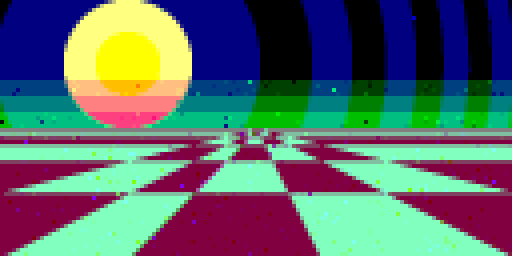
\includegraphics[scale=0.96]{img/prog_res/qss-512-6.png}
	\end{center}
	\captionsetup{justification=centering}
	\caption{Результат работы квантового алгоритма, 512х256, 6 итераций увеличения комплексной амплитуды, размер сабпикселя 4х4}
	\label{img:example_02}
\end{figure}

\begin{figure}[H]
	\begin{center}
		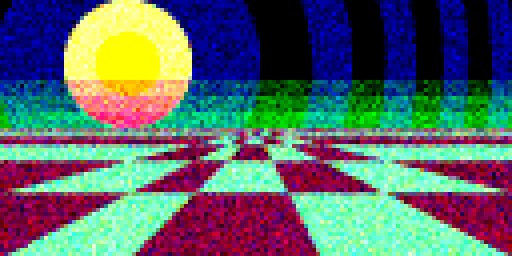
\includegraphics[scale=0.96]{img/prog_res/monte-carlo-512.png}
	\end{center}
	\captionsetup{justification=centering}
	\caption{Результат работы алгоритма Монте -- Карло, 512х256, размер сабпикселя 4х4}
	\label{img:example_01-mc}
\end{figure}

\begin{figure}[H]
	\begin{center}
		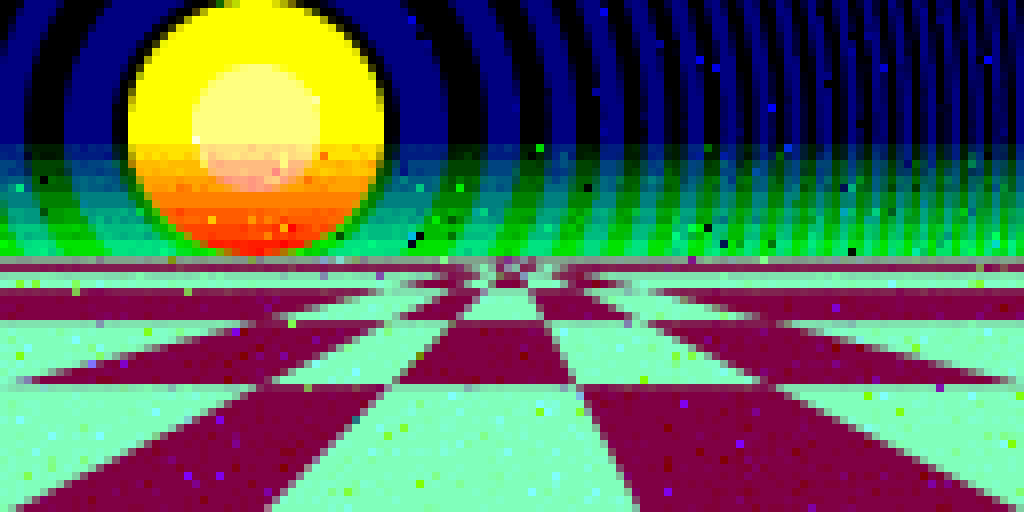
\includegraphics[scale=0.48]{img/prog_res/qss-1024-6.png}
	\end{center}
	\captionsetup{justification=centering}
	\caption{Результат работы квантового алгоритма, 1024х512, 6 итераций увеличения комплексной амплитуды, размер сабпикселя 9х9}
	\label{img:example_03}
\end{figure}

\begin{figure}[H]
	\begin{center}
		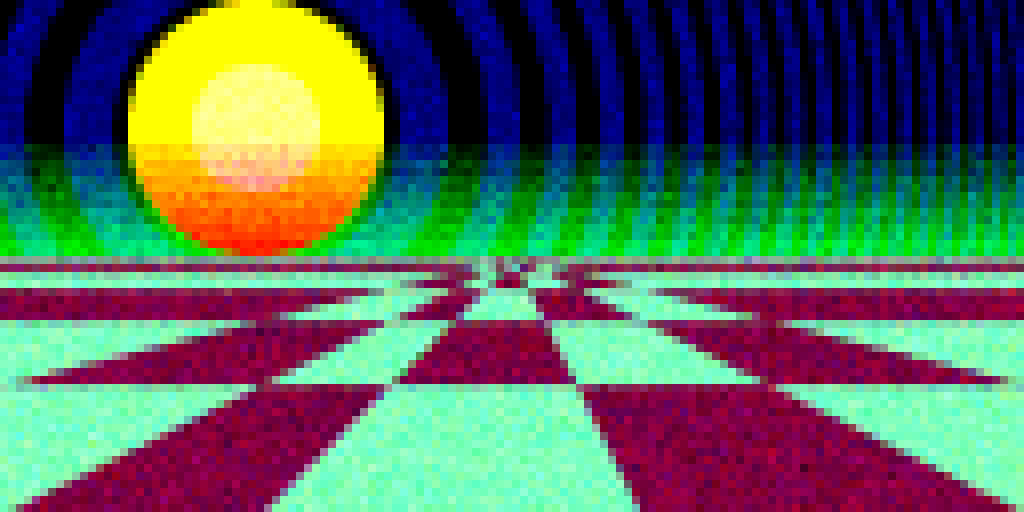
\includegraphics[scale=0.48]{img/prog_res/monte-carlo-1024.png}
	\end{center}
	\captionsetup{justification=centering}
	\caption{Результат работы алгоритма Монте -- Карло, 1024х512, размер сабпикселя 9х9}
	\label{img:example_03-mc}
\end{figure}

\section{Постановка эксперимента} 

\subsection{Цель эксперимента}

Целью эксперимента является проведение трех независимых сравнений результатов работы программного обеспечения:

\begin{itemize}
	\item сравнение уровня шума на изображении синтезируемого алгоритмом Монте -- Карло и квантовым алгоритмом;
	\item сравнение характера шума на изображении синтезируемого алгоритмом Монте -- Карло и квантовым алгоритмом;
	\item сравнить вычислительные сложности алгоритма Монте -- Карло и квантового.
\end{itemize}

\subsection{Сравнение уровня зашумленности}

Сравнить уровень зашумленности двух синтезируемых изображений можно расчитав средний процент ошибки на каждый пиксель.

Результаты сравнения уровня зашумленности для изображений разных размеров приведены в таблице \ref{tab:noise}. Во втором и третьем столбце таблицы расположены средние проценты ошибок для рассматриваемых реализаций алгоритмов. Размер сабпикселя равен 4х4.

\begin{table}[h!]
	\caption{Сравнение уровня зашумленности для классического и квантового алгоритма избыточной выборки.}
	\label{tab:noise}
	\begin{center}
		\begin{tabular}{|c | c | c|} 
			\hline
			Размер изображения & Классическая выборка & Квантовая выборка \\  
			\hline
			64x64 & 3\% & 2\%  \\
			\hline
			128x128 & 4\% & 2\% \\
			\hline
			256x256 & 4\% & 3\% \\
			\hline
			512x512 & 4\% & 3\% \\
			\hline
			1024x1024 & 4\%  & 4\% \\
			\hline
		\end{tabular}
	\end{center}
\end{table}

\subsection{Сравнение характера шума}

Из-за того что в квантовом случае пиксели получаемого изображения могут быть либо идеальными, либо крайне зашумленными \cite{PQC-classic}, сравнение характера шума  изображения можно провести подсчитав процент идеальный пикселей от всего изображения. 

В таблице \ref{tab:noise_02} приведено сравнение характера шума для разных размеров изображения. Размер сабпикселя равен 4х4.

\begin{table}[h!]
	\caption{Сравнение характера шума классического и квантового алгоритма избыточной выборки.}
	\label{tab:noise_02}
	\begin{center}
		\begin{tabular}{|c| c | c|} 
			\hline
			Размер изображения & Классическая выборка & Квантовая выборка \\  
			\hline
			64x64 & 58\% & 88\%  \\
			\hline
			128x128 & 71\% & 78\% \\
			\hline
			256x256 & 63\% & 75\% \\
			\hline
			512x512 & 62\% & 73\% \\
			\hline
			1024x1024 & 61\% & 70\% \\
			\hline
		\end{tabular}
	\end{center}
\end{table}

\subsection{Сравнение вычислительной сложности алгоритмов}

Для того чтобы оценить время выполнения алгоритмов, нужно вывести их сложность. Вычислительная сложность алгоритма Монте -- Карло напрямую зависит от размера изображения и составляет $O(n)$ \cite{mc-complexity}. На основе изложенного алгоритма в разделе \ref{qss-algo}, выведем сложность выполнения квантового алгоритма избыточной выборки. При этом, примем что все квантовые операции выполняются за $O(1)$. 

Опираясь на описание квантового алгоритм избыточной выборки из раздела \ref{qss-algo}, построчно рассчитаем его сложность:

\begin{itemize}
	\item перевести все пиксели холста в состояние 1 -- O(1) (реализуется с помощью операции смены фазы, см. раздел \ref{qphase});
	\item сформировать и заполнить квантовую поисковую таблицу -- $O(n * k)$, где k -- глубина итераций усиления комплексной амплитуды. Так как $k$ -- константа (см. раздел \ref{yka}), мы имеем право отбросить эту константу \cite{computation-complexity}, получая конечную сложность формирования таблицы $O(n)$;
	\item посчитать количество инвертируемых пикселей (для каждого пикселя холста) -- $O(n^2)$;
	\item заполнить соответствующую ячейку карты достоверности (для всей таблицы) -- $O(n^2)$.
\end{itemize}

Итоговая вычислительная сложность квантового алгоритма избыточной выборки составляет (\ref{for:qss-complexity}):

\begin{equation}
	\label{for:qss-complexity}
	c * (O(1) + O(n) + O(n^2) + O(n^2)) = O(n^2)
\end{equation}
где $c$ -- число цветов колоризации. Так как это число является константой (см. раздел \ref{color}), в конечном счете мы можем откинуть его \cite{computation-complexity}.

\section*{Вывод}

Как и ожидалось, уровень зашумленности изображения примерно равен как для классической выборки, так и для квантовой. Так, например, средний процент ошибки на пиксель при размере синтезируемого изображения 512х512 для квантового алгоритма составляет 3\%, а для классического 4\% соотвественно.

Квантовая выборка на маленьких размерах изображения выдает большой процент идеальных пикселей. Например, для изображения размером 64х64 количество идеальных пикселей составляет 88\% от всего изображения. Но, с увеличением изображения этот процент незначительно падает, и уже на размере изображения 512х512 составляет 73\%. Несмотря на это, классическая выборка даже в самом лучшем случае не добивается такого результата -- ее лучший результат 71\% идеальных пикселей для размера изображения 128х128. Квантовый алгоритм генерирует на 10\%..30\% идеальных пикселей больше, чем его классический аналог, из чего можно сделать вывод о сильных различиях в характере шума.

Была оценена вычислительная сложность квантового алгоритма избыточной выборки $(O(n^2))$. Исходя из того факта, что сложность выборки Монте -- Карло составляет $O(n)$, можно сделать что квантовый алгоритм будет проигрывать по времени работы классическому аналогу даже на настоящем квантовом компьютере.